 % Useful: http://docs.latexlab.org

\documentclass[11pt]{article}
% used by \maketitle :
\title{DarkChat: a light weight, [almost] server-free, push-based robust p2p network with a chat payload}
\author{Nathan Griffith and Ahmet Aktay}
\date{May 12, 2010}
% used by \begin{code}:
\usepackage{fancyvrb}

\usepackage[utf8]{inputenc}
\usepackage[usenames,dvipsnames]{xcolor}
\usepackage{fullpage}
\usepackage[upright]{fourier}
\usepackage{tkz-graph}
\usetikzlibrary{arrows}


\DefineVerbatimEnvironment{code}{Verbatim}{fontsize=\small}
\DefineVerbatimEnvironment{example}{Verbatim}{fontsize=\small}
\newcommand{\ignore}[1]{}

\begin{document}
\maketitle % automatic title!

\section{Abstract}

The purpose of this project is to create a protocol for clients on a network to function with very little dependence on a server. In the case of \emph{DarkChat}, the clients function as 'chat' clients. The clients are able to communicate with each other information such as `online'/`offline' state and lists of contacts, with little-to-no interaction with the server.

While \emph{DarkChat} relies on a multi-threaded approach, and also makes no use of authentication, implementation decisions such as this have been made independently of the underlying protocol. As such, the protocol could be implemented in any number of ways, and this is meant as merely one example. The event-based stateless nature of the protocol makes an asynchronous IO implementation very lucrative in terms of resource utilization.

\section{Clients and Servers}

The `Client' class has been built as a wrapper for the messaging and interface classes, putting them all together into one usable chat client. Note that the term `client' is slightly misleading, as with the inclusion of a simple flag, a client can function as a server with very few implementation changes. It is possible that this could be reduced even further, such that servers could simply act as `super-clients' which store information about the entire network, instead of about only their nearby edges and nodes.
In either case, the only purpose of the server is to act as a secondary or backup repository for storing information about the network. Once the network is fully operational, the server is not needed, as long as enough clients remain online that one cluster of edges does not become separated from any other. In other words, the server is a client that has been flagged as having access to greater bandwidth and resources, and can shoulder a bigger burden in maintaining network topology. It has no additional logic and hence is not a liability.

\subsection{Usage: Parameters}

When executing the client, a number of parameters can be passed. WIth the exception of `username' (`-u'), all parameters will revert to default values if none is specified:

\begin{code}
-p [port number, for accepting incoming communication]
-t [the default number of listening threads]
-u [the username of the client]
-sip [ip address of known server]
-sp [port number of known server]
-s (server flag, specifying that this instance of DarkChat is a server)
\end{code}

Note that there is currently no reliable centralized server, so in the actual case of starting a network running from scratch, it would be best to ensure that a server is running, and specify the server ip and port for each client. Once the clients are online and have contacted each other, one need only use a macro to contact a currently online client.

\subsection{Usage: Macros}

Once the client has been started, a number of macros have been made available to give the user control:

\begin{code}
  \help
   -Display this dialog
  \chat <username>
   -Switch to conversation with <username>
  \users
   -See a list of KNOWN users (online or off)
  \online
   -See a list of known, ONLINE users
  \offline
   -See a list of known, OFFLINE users
  \add <username>
   -Attempt to add username to list of known users
  \ping <ip> <port>
    -Attempt to ping the ip at the given port
    -If no port is specified, the current instance's incoming will be used
  \explode
    -ask every adjacent node to notify every adjacent node that this user in online at this address.
  \quit or \exit
   -Leave the program gracefully
\end{code}

Note that these are made available before the client has necessarily made successful contact with a server, allowing one to use the `\textbackslash ping' macro to manually connect to another client or server, or begin chatting with users whose nodes are remembered from previous executions.

Once a connection has been made, information about offline and online users should propagate across the network and to the client, at which point the macros `\textbackslash online', `\textbackslash offline', and `\textbackslash users' will provide useful information.

To communicate with an online user, one need only use the `\textbackslash chat' macro (followed by the user's name) to start a new chat session with that user. From that point on, any line of text that is entered and doesn't start with a macro `\textbackslash' will be sent to \emph{all online sessions} associated with the receiver's username.\footnote{Currently there is no way to chat with \emph{only one} session if a user is logged into multiple.}

This accommodation of multiple sessions per user allows another form of robustness. All protocol messages, not just active chats have this property. That is, any transactions between an en user and another will be mirrored in any other nodes with the same user. Even if one node disconnects, the other can carry on the conversation, and more importantly, maintenance of the topology.

As an expensive proof-of-concept of how the network could propagate detailed information about nodes using our serverless sustaining push scheme, the `\textbackslash explode' macro will push out and propagate an address declaration from the original node to all its adjacent nodes, \emph{via all short paths}. This will ensure that every node in that zone will have a significant (read: almost certain) chance at being sent the ping by the original node. With little optimization, the node could broadcast (vicariously) its declaration to a set of users within a short bounded distance without much unneeded redundancy. If each node has n links going out, notifying a sphere of nodes with distance $\leq$ 2, would notify n$^2$ users in O(n$^2$) time. The node would then get n$^2$ responses back, acquiring information about n$^2$ users. In general, network traversal becomes cheap as long as we focus on short-range clusters, which occur naturally in social communications, and also can reflect the physical hardware topology of the network (users in a cluster are more likely to be `stranded' in the same island in the event of network failure.) Hence streamlined versions of actions like `\textbackslash explode' can keep the topology regenerating without relying on the (potentially offline) central server.

\section{The Algorithm}

While the details of the `Chat' client is useful in understanding some aspects of this algorithm, the true implementation has been abstracted from the end-user. Therefore, to understand the intent behind this project, a deeper explanation of the algorithm is required.

\subsection{The Network}

Instead of picturing the network in terms of `users' and `buddies' and `servers,' as one might with some types of chat implementations, one can also see it very simply as an undirected graph composed of nodes and edges. Each node represents a `client,' and each edge represents a direct, two-way association between two clients.\footnote{In the context of `chat,' adjacent nodes might represent ``buddies,'' but it's important to think of them abstractly.}

\begin{figure}
  \caption{An example network configuration}
  \begin{center}
  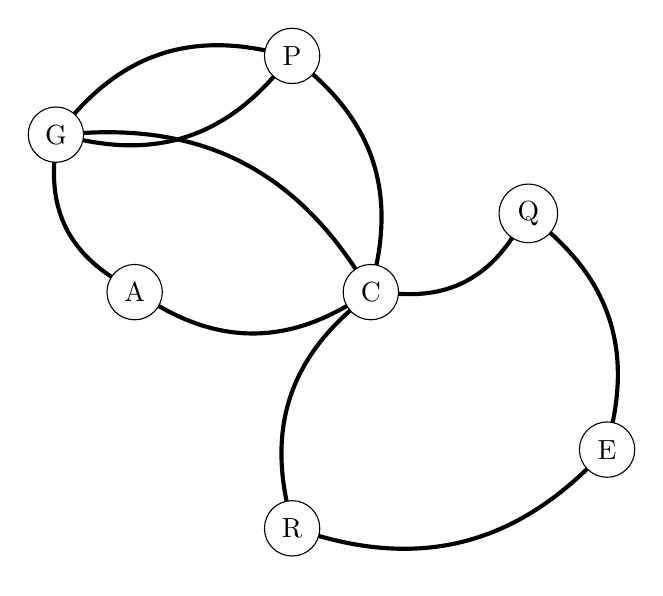
\begin{tikzpicture}
    \tikzstyle{VertexStyle}=[shape = circle, fill = white, minimum size = 20pt, text = black, draw]
    \SetUpEdge[lw         = 1.5pt,
                       color      = black,
                     labelcolor = white,
                      labeltext  = red,
                      labelstyle = {sloped,draw,text=blue}]
   \tikzstyle{EdgeStyle}=[bend left]
   \Vertex[x=0, y=4]{G}
   \Vertex[x=1, y=2]{A} 
   \Vertex[x=3, y=5]{P}
   \Vertex[x=4, y=2]{C}
   \Vertex[x=6, y=3]{Q}
   \Vertex[x=7, y=0]{E}
   \Vertex[x=3, y=-1]{R}
   \Edges(A,G,P,C)
   \Edges(Q,E,R,C,A)
   \Edges(P,G,C)  
   \Edges(Q,C)
  \end{tikzpicture}
  \end{center}
\label{graph}
\end{figure}

As shown in {\bf Figure \ref{graph}}, a network graph might look like one or more clusterings of nodes\footnote{This could be particularly true in the case of a `chat' client.}. In the \emph{DarkChat} implementation, each node is required to keep track of all nodes that are within two edge traversals.

When, for instance, a node is to add or update information about itself, it sends a notification to all nodes in its list of relevant nodes. This means that if, for instance, \emph{Node R} and \emph{Node E} have lost their connection to each other\footnote{This might happen if they have both changed IP addresses since their last communication}, they could rely on either \emph{Node C} or \emph{Node Q} to provide one of the required locations\footnote{Note that, of two nodes, only one need know the other's location in order for a connection to be established. In the case of \emph{E} and \emph{R}, as soon as \emph{Node E} sends a message to \emph{Node R}, the location of \emph{Node E} has been revealed.}.

Notice that \emph{Node C} is directly paired with all but \emph{Node E}, and even then \emph{E} and \emph{C} are within two edge traversals. This is a good example of a node with \emph{server-like} capabilities for this netork graph. However, since \emph{C} is in fact a client, this is a good example of the ways in which a server-free graph can still maintain robust and redundant connections for sending and recieiving updates.

THe final aspect of this graph worth noting is the fact that no server is shown. Presumably, all nodes would also be connected to some centralized server. However, under many normal conditions, this server would not be required. Only in cases where nodes are completely stranded would they \emph{need} to poll the server in order to maintain an accurate representation of their surrounding nodes. One such case might be if \emph{Node R} and \emph{Node E} are attempting to communicate with each other, and \emph{Node C} and \emph{Node Q} are both offline. As such, the more interconnected the clusters of nodes, the `healthier' the network.\footnote{This does not necessarily imply that the entire network is very interconnected, though this could also be the case. Instead, the `interconnectedness' implies only that many connections are shared within each cluster of nodes, of which there could be many.}

\subsection{The Status}

While each node's online/offline status is stored at each linked node, even offline nodes are remembered in session variables and kept. Since most end-users use the same network connections consistently through time (static IP at home and work,) this information can be used to bootstrap the connectivity of the network without invoking the central server. A balance has to be struck between iterating through (potentially useless) old addresses for nodes when attempting to reach them, and pruning the oldest away to streamline the process. In this implementation, we prune the list of sessions on demand to a desired length, favoring online sessions (however many) over recent offline ones.
   
\subsection{The Protocol}

Clients make use of a limited number of message types to receive the information they need. The message sending and respond happens without state.

\begin{description}
\item \emph{declareOnline} - sends a message to a specified user (all sessions thereof,) notifying it of its address and availability.
\item \emph{declareOffline} - declares to the specified user that it is going offline.
\item \emph{requestPing} - sends a user a request for it to deliver a \emph{declareOnline} message to a target. Helps restore missing links.
\item \emph{requestUserList} - asks a user to send it a list of who the originator of the request is linked to. Helps bootstrap the network.
\item \emph{deliverKnownList} - in response to a user list requests, sends back a list of users that it knows the requesting user is linked to. When processed by a server, the list is complete. Otherwise, multiple adjacent users might have to be polled to build out the set.
\end{description}

\section{Use Cases}

\emph{DarkChat} is NOT for high payload bandwidth, frequent-topology-shift-ridden networks. It saves bandwidth for the \emph{server} by distributing the traffic workload to the clients. We believe that in many real world cases, the payload is light enough and the added redundancy and synchronicity would be wroth enough that a fleshed out \emph{DarkChat} implementation would have advantages outweighing the disadvantages.

\emph{DarkChat} has the useful property of running in its failure mode when possible \emph{even when the system is intact}. This creates a significant advantage for the protocol: Its failsafes, backups and system load are tested (and ideally refined) during regular uptime activity, hopefully shaping the robustness into a tested and true practicality rather than an abstract potential benefit.



When compared to heavy-hitting infrastructures like Microsoft's Partition and Recovery Service, we see that \emph{DarkChat}-type protocols leave a lot to be desired in terms of precise and 100\% accurate recovery of data. On the other hand, systems like PRS have the advantage of designing the hardware and network layout from the ground up, while \emph{DarkChat} is built to run on available (non-enterprise) network architectures. In the event of failure, while PRS will focus on recovering data integrity, DarkChat will aim to maximize connectivity across its network topology. To this end it sacrifices the requirement that everything be restored, or that all nodes stay fully synchronous. This gives the DarkChat protocol the flexibility to withstand catastrophic failures (for some definitions of withstand.) Consider a hypothetical use: coordination amongst first responders in case of an emergency. The nodes that want to communicate will be physically close, and getting \emph{any} message through in any manner possible will be the only priority. The network DarkChat is running on might fragment into disconnected pieces entirely, but each piece will still maintain its internal topography as intact as possible and continue to ping the `missing' users in case connectivity has been restored. For cases in which tainted, contaminated and fragmented function is still significantly better than none, DarkChat and protocols like it could be more handy than PRS like solutions, even if the payload is large chunks of data rather than light chat messages.

\section{Possible Optimizations}
scaling for bandwidth
   
message identifiers
   
combined requests

   
\begin{thebibliography}{1}

  \bibitem{prs}
    Atul Adya, John Dunagany, Alec Wolman,
    \emph{PRS: A Reusable Abstraction for Scaling Out Middle Tiers in the Datacenter}.
    Microsoft Research; Microsoft Corporation,
    2008.
\end{thebibliography}
\end{document}             % End of document.

